% !TEX root = ../thesis.tex

\chapter{Neural Style}
\label{chap:system}

\cleanchapterquote{Sometimes a problem that initially looks hopelessly complicated turns out to have a surprisingly simple solution.}{Nick Bostrom}{(Superintelligence: Paths, Dangers, Strategies)}


% ------------------------------------------------------------------------------

In this chapter, we finally present and explain \citeauthor{Gatys2015B}'s approach to separation of style and content with the neural style algorithm \cite{Gatys2015B}.

We have seen in Chapter~\ref{chap:context} how the field of non-photorealistic rendering has tried for a long time to produce techniques that better separated style and content in order to produce more compelling results in style transfer tasks.
These techniques focused more and more towards capturing larger-scale patterns, which is something convolutional neural networks (CNNs) trained in object recognition have proved to excel at.
Recent efforts in understanding CNN have delivered visualization techniques that can produce compelling images from the internal representations of deep neural networks.
Neural style relies both on CNN and visualization techniques to give a holistic approach to separation of style and content, as we will see next.

The neural style algorithm is a novel approach to style transfer that is able to manipulate content and style independently.
Some examples of the results achieved by their algorithm can be seen in \autoref{sub:system:examples}.

\begin{figure}[!htb]
  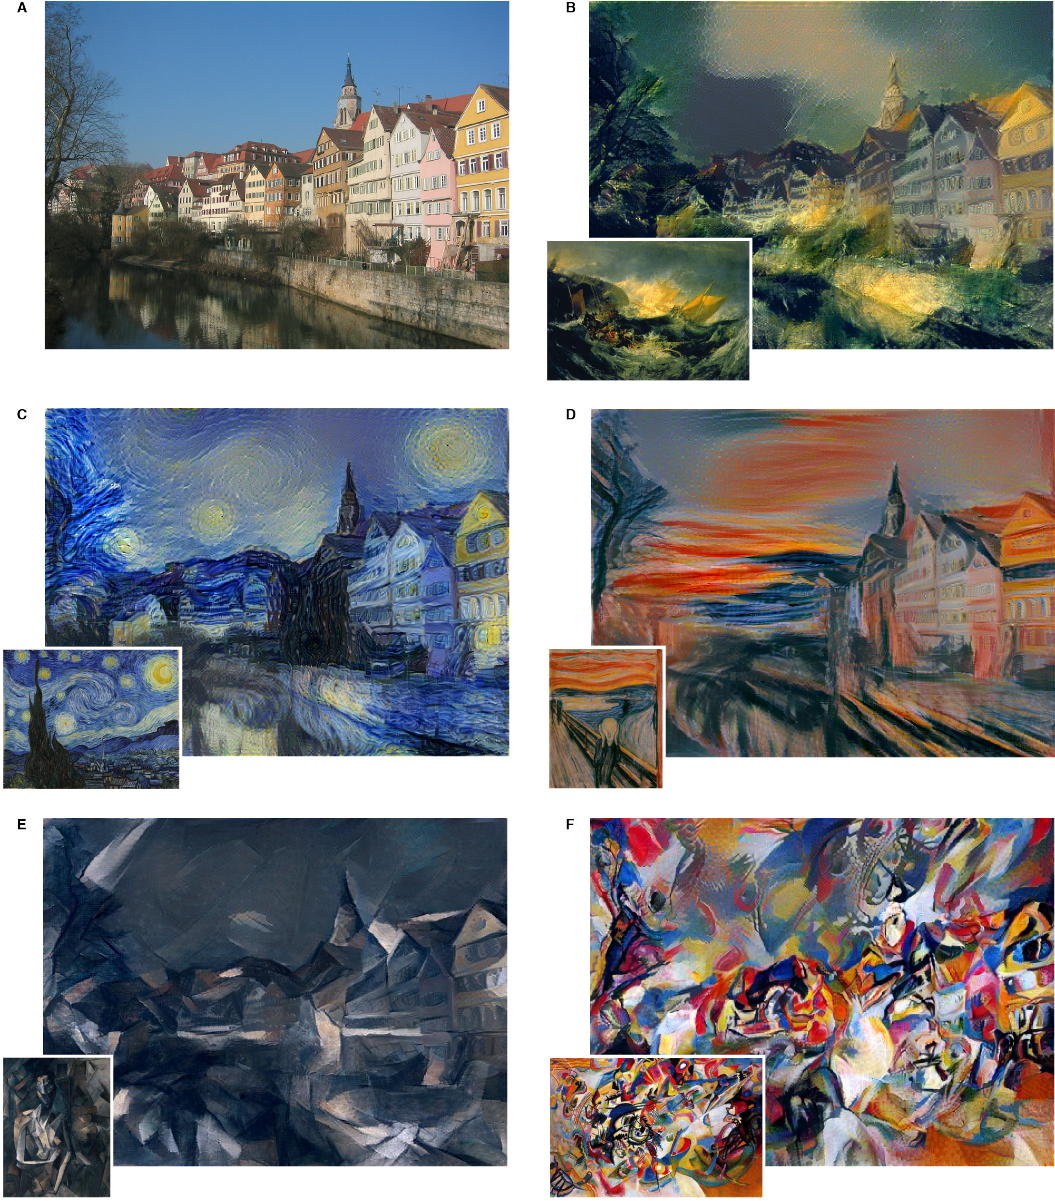
\includegraphics[width=\textwidth]{gfx/neural-style-examples}
  \caption{
    Images synthesized using the neural style algorithm \cite{Gatys2015B}.
    In \textbf{A}, the original photograph, depicting the Neckarfront in T\"ubingen, Germany, (shot by Andreas Praefcke).
    The style is applied from different artworks, shown in the bottom left corner of each panel.
    \textbf{B} \emph{The Shipwreck of the Minotaur} by J.M.W. Turner, 1805.
    \textbf{C} \emph{The Starry Night} by Vincent van Gogh, 1889.
    \textbf{D} \emph{Der Schrei} by Edvard Munch, 1893.
    \textbf{E} \emph{Femme nue assise} by Pablo Picasso, 1910.
    \textbf{F} \emph{Composition VII} by Wassily Kandinsky, 1913.
  }
  \label{sub:system:examples}
\end{figure}

In these examples, we observe how the style from several artworks is transferred to an original photograph.
The content of the photograph, its global arrangement, is consistently preserved while the style of the artworks, color, patterns, and local structures, is blended seamlessly.
Previous approaches mainly rely on non-parametric techniques or directly operate on the pixel representation of images, as we saw previously.
Instead, neural style, by using a CNN trained in object recognition is able to: on the one hand extracting content patterns of arbitrary size in an image, and on the other hand applying deep visualization techniques to perform manipulations directly in those feature spaces, providing not a robust but also flexible style transfer method.
From the perspective of style transfer as an artistic rendering tool, it is desirable for the algorithm to provide a sufficiently rich space of results to explore \cite{Ashikhmin2003}, and neural style easily surpasses any of the techniques seen before.
Further in this chapter (\autoref{fig:system:results}) we show how every pair of content-style images emphasis on content and style can be combined in multiple ways.

As discussed in Chapter~\ref{chap:intro}, style has traditionally received little attention in pattern recognition tasks in machine learning \cite{Karayev2014}.
Some attempts were done before in separation of style and content \cite{Tenenbaum2000,Elgammal2004}, their reach was limited to much simpler input, such as characters in different handwriting or faces with slightly different poses.
Neural style presents a completely novel approach to separation of style and content and it happens to require only a few adjustments on a CNN already trained for object recognition, as we will see next.


% ------------------------------------------------------------------------------

\section{Method}
\label{sec:system:method}

Neural style, simply put, takes two image sources: a photograph and an artwork, extracts the content from one and the style from the other, and generates a new image that matches both simultaneously.
The whole algorithm relies on a CNN already trained in object recognition to extract content and style from features found in source images.

\citeauthor{Gatys2015B}'s particular implementation uses VGG-Network \cite{Simonyan2014}, a CNN already trained in object recognition.
VGG-Network was designed and trained by the Visual Geometry Group at the University of Oxford with the goal of evaluating the performance of networks with increasing depth and it managed to score top results in ImageNet Challenge 2014.
The network achieved best results in between 16 and 19 weight layers with an architecture of convolutional filters with a very small receptive field (${3}\times{3}$, the smallest that can capture the notion of left/right, up/down and center) stride set to 1 pixel, and zero-padding to 1 pixel as well to preserve the original resolution of the input after the convolution.
Subsampling is performed by 5 max-pooling layers, inserted after some of the convolutional layers, over a ${2}\times{2}$ pixel window with stride set to 2 pixels so that the filter does not have overlapping input.

The VGG-Network implementation in Caffe framework is available under Creative Commons Attribution License \cite{Simonyan2014web}.
Among the 19-layer VGG-Network, neural style uses all 16 convolutional and 5 pooling layers, but none of the fully-connected layers, since classification is not required.
Max-pooling is replaced by average pooling because it produces a smoother gradient flow \cite{Boureau2010} and it results in cleaner synthesized images.
Lastly, for practical reasons, the weights in the networks are rescaled such that the mean activation of each filter over images and positions is equal to one.
Rescaling weights in this manner is always possible without affecting the output of the CNN when the activation functions are normalized with a ReLU layer like is the case in VGG-Network.

In a bit more detail, these are the algorithm's main stages: 1) both images get processed by the VGG-Network to produce their feature spaces, 2) content and style are extracted from those, and finally 3) a new image that matches them both is generated through backpropagation.

We will focus next on what we mean by content and style exactly and then how VGG-Network can synthesize new images that match content or style representations from a source image.
At the end, it will be obvious how it is possible to transfer the style using the neural style algorithm.


\subsection{Feature Representations}
\label{sub:system:method:representations}

Content and style of an image in neural style is characterized making use of the feature space produced by the VGG-Network.
If we remember the introduction on CNNs discussed in \autoref{sec:theory:convnets}, an original input gets transformed by filters defined in each layer as it moves across the network during the feed-forward phase.
To be more precise, a layer produces as many feature maps as filters it defines, each one of them highlighting different features of the input and represented by neural activations.
Spatially, we can imagine the output from a layer as a volume in which each slice is a feature map where neuron responses are arranged in 2D grids.
In image recognition tasks, each feature map is actually another image where pixels are active wherever the feature captured by the associated filter is present.

\paragraph{Content Representation}
We can also understand it the other way around, perceiving neural activations at a certain layer as an abstract representation of the original input image.
As a result of the VGG-Network having been trained in object recognition, its learned filters capture spatial information of the original input image, and thus, we can talk of the neural activations from a CNN layer as the content representation.
Formalizing it for an input image $\vec{x}$, let $l$ be a layer that applies $N_l$ different filters and produces $N_l$ feature maps of size $M_l$, where size is defined by the resolution ${height}\times{width}$ of the feature maps.
Vectorizing the feature maps, the total neural response at layer $l$ can be stored in a 2D matrix $F^l \in \mathbb{R}^{{N_l}\times{M_l}}$ where $F^l_{ij}$ is the feature activation for the $i^{th}$ filter at neuron $j$.

\begin{equation}
  F^l =
  \underbrace{
    \begin{bmatrix}
      F^l_{11}   & F^l_{12}   & \dots  & F^l_{1M_l} \\
      F^l_{21}   & F^l_{22}   & \dots  & F^l_{2M_l} \\
      \vdots     & \vdots     & \ddots & \vdots   \\
      F^l_{N_l1} & F^l_{N_l2} & \dots  & F^l_{N_lM_l}
    \end{bmatrix}
  }_{\text{vectorized feature maps}}
  \begin{matrix*}[l]
    \leftarrow & \text{filter } 1 \\
    \leftarrow & \text{filter } 2 \\
    \vdots                     \\
    \leftarrow & \text{filter } N_l
  \end{matrix*}
\end{equation}

\paragraph{Style Representation}
VGG-Network, as stated before, was not trained in any kind of style recognition task, so it is clear there is no style representation of any sort directly available in the network.
Nonetheless, \citeauthor{Gatys2015A} described in a previous work \cite{Gatys2015A} a method to build a style representation on top of the content representations without having to modify the network.
While the concept of content representation is somewhat intuitive to comprehend, style representation will require us to take a short detour to explain what we mean with style and what we expect its representation to be.

\citeauthor{Gatys2015A} approach style as a texture.
Texture synthesis tries to extract a texture model from an initial example so that arbitrary new samples of textures can be produced from it.
The quality of the model is normally evaluated by how hard it is for human inspection to distinguish between original and generated.
A texture model cannot be described by its exact pixel representation, rather a texture model must be uniquely described by statistical measurements, referred to as summary statistics, as was originally proposed by \citet{Julesz1962}.
We can understand this better by looking at \autoref{sub:system:method:style-reconstruction:texture}, showing a randomly generated image with 4 levels of brightness where a different texture has been applied on either half.
On the one hand, it illustrates how textures are independent of exact pixel representation as the randomly generated grid does not affect our ability to distinguish both textures.
On the other hand, it proves summary statistics are a better metric to distinguish one pattern from another.
This means that, within a texture model, any image that presents the same summary statistics as another, although having a different exact representation, can be considered the same texture.

\begin{figure}[htb]
  \begin{subfigure}[b]{0.5\textwidth}
    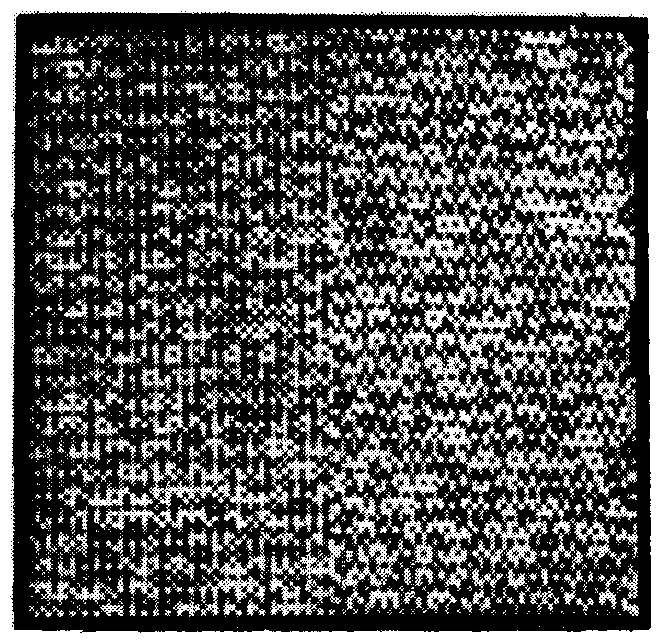
\includegraphics[width=\textwidth]{gfx/texture-1}
    \caption{Two-texture image}
    \label{sub:system:method:style-reconstruction:texture-1}
  \end{subfigure}
  \hfill
  \begin{subfigure}[b]{0.5\textwidth}
    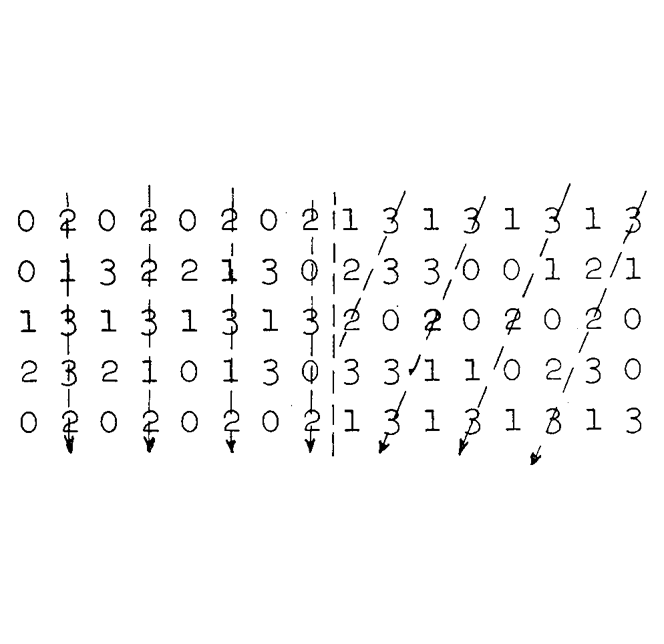
\includegraphics[width=\textwidth]{gfx/texture-2}
    \caption{Texture pattern generation}
    \label{sub:system:method:style-reconstruction:texture-2}
  \end{subfigure}
  \caption{Pattern discrimination \cite{Julesz1962}.
    On the left (a), an image with two different textures clearly visible.
    On the right (b), the pattern used to generate different textures on both halves of the image.
    Numbers represent the level of brightness and those outside of the arrows are randomly distributed.
    While no two regions on either half of the image are the same (brightness random distribution), the underlying patterns existing on each half (arrows) make them clearly distinguishable.}
  \label{sub:system:method:style-reconstruction:texture}
\end{figure}

Texture synthesis was later inspired by human visual systems, using Gabor filters for edge detection, which proved to be very similar to the human visual system \cite{Heeger1995,Portilla2000} and statistical measurements in these cases were taken over Gabor filter responses rather than on image pixels.
Results presented by \citet{Portilla2000} are probably still the best produced to date \cite{Gatys2015A}, but the method required careful handcrafting summary statistics that would result in good texture models.
Because of this, \citeauthor{Gatys2015A} argued \citeauthor{Portilla2000}'s method fails to generalize the full extent of natural textures and proposed in \cite{Gatys2015A} a method that combines the use of summary statistics with the feature space of a CNN already trained in object recognition, which fully models the human visual system.

Picking up again the analogy between textures and style, the summary statistic of the texture model is what we refer to as the style representation.
Since textures models are per definition stationary, the style representation must discard the spatial information existing in feature maps while keeping the notion of patterns.
One way to achieve it is by calculating the correlations between features maps in a CNN layer.
We can, therefore, formalize the style representation of an image $\vec{x}$ as a set of per-layer feature correlations $\{G^1, G^2, \dots, G^L\}$, where per-layer feature correlations are stored in 2D Gram matrixes $G^l \in \mathbb{R}^{{N_l}\times{N_l}}$ \cite[Theorem~7.2.10]{Horn2012}:

\begin{equation}
  G^l =
  \begin{bmatrix}
    G^l_{11}   & G^l_{12}   & \dots  & G^l_{1N_l} \\
    G^l_{21}   & G^l_{22}   & \dots  & G^l_{2N_l} \\
    \vdots     & \vdots     & \ddots & \vdots   \\
    G^l_{N_l1} & G^l_{N_l2} & \dots  & G^l_{N_lN_l}
  \end{bmatrix}
\end{equation}

Being $G^l_{ij}$ the inner product between the vectorized feature maps $i$ and $j$ in layer $l$, representing their degree of correlation:

\begin{equation}
  G^l_{ij} =
  \begin{bmatrix}
    F^l_{i1} & \dots & F^l_{iM_l}
  \end{bmatrix}
  \begin{bmatrix}
    F^l_{j1} \\
    \vdots \\
    F^l_{jM_l}
  \end{bmatrix}
  = \sum_k F^l_{ik}F^l_{jk}
\end{equation}

Having defined content and style representations we can now move to discussing how they can be used to produce new images.
\citeauthor{Gatys2015B} refer to this process feature reconstruction.


\subsection{Feature Reconstruction}
\label{sub:system:method:reconstructions}

In neural style algorithm, feature reconstruction is the process of visualizing some feature representation of an original input image.
The visualization is, in fact, a new image $\vec{x}$ that must be generates so that either its content representation or its style representation matches that of the original input image.
We will talk about \emph{content reconstruction} when the new image $\vec{x}$ is generated so that matches the content representation and \emph{style reconstruction} when it does so with the style representation.
The strategy to generates the new image $\vec{x}$ is approaching the task as an optimization problem very much like backpropagation, as we will see next.

\paragraph{Content reconstruction}
Starting from a random white noise image $\vec{x}$, we want to transform it so that it becomes the image $\vec{x}$ whose content representation is the same as the original photograph $\vec{p}$ at a certain layer $l$.
It is then the difference between content representations of $\vec{x}$ and $\vec{p}$ what we need to minimize.
So, let $P^l$ and $F^l$ be the content representations of the original photograph $\vec{p}$ and the generated image $\vec{x}$, respectively, in layer $l$, we define the loss function to be minimized as the squared error between the two representations:

\begin{equation}
  \mathcal{L}_{content}(\vec{p}, \vec{x}, l) = \frac{1}{2} \sum_{i,j}(F^l_{ij}-P^l_{ij})^2
\end{equation}

With this loss function we want to ultimately modify the white noise image $\vec{x}$, which can be perceived as the content representation at the input layer $l = 0$, so we can say we want to find the partial derivative of the loss with respect to the content representation such as:

\begin{equation}
  \Delta \vec{x} =
  \frac{\partial \mathcal{L}_{c}}{\partial \vec{x}} =
  \frac{\partial \mathcal{L}_{c}}{\partial F^0}
\end{equation}

Which generalized for any layer $l$ with the chain rule can be analytically calculated for every neuron as:

\begin{equation}
  \mathcal{L}^l_{ij} =
  \frac{\partial \mathcal{L}_{c}}{\partial F^l_{ij}} =
  \begin{cases}
    (F^l - P^l)_{ij} & \text{if } F^l_{ij} > 0 \\
    0                & \text{if } F^l_{ij} < 0
  \end{cases}
\end{equation}

We can then apply standard error backpropagation \cite{Orr2008} as depicted in \autoref{fig:system:method:feature-reconstruction} to calculate the gradients for each pixel of the white noise image $\vec{x}$.
With them, we can adjust $\vec{x}$ until its content representation matches that of the photograph $\vec{p}$ at layer $l$.

\begin{figure}[htb]
  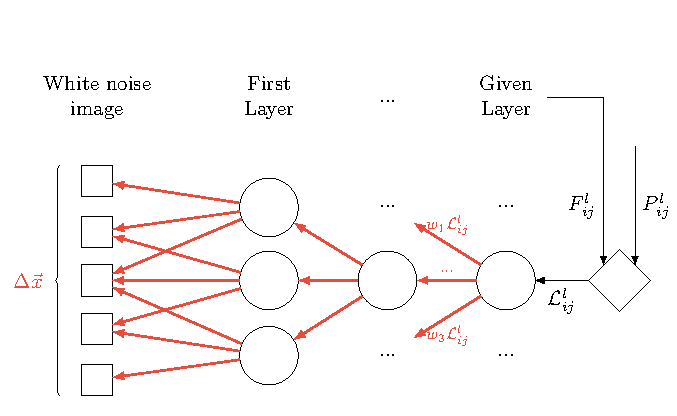
\includegraphics[width=\textwidth]{tkz/feature-reconstruction}
  \caption{
    Content reconstruction with standard backpropagation.
    The content loss $\mathcal{L}^l_c$ is numerically calculated for each neuron in a given layer $l$ from the content representation $F^l$ and $P^l$, resulting from the feed-forward pass of the white noise image $\vec{x}$ and the photograph $\vec{p}$ respectively.
    The calculated loss is backpropagated through the whole network until it reaches the first layer.
    The gradients $\Delta \vec{x}$ for adjusting the white noise $\vec{x}$ are calculated in the same way as if the input layer is a CNN layer.
  }
  \label{fig:system:method:feature-reconstruction}
\end{figure}

\paragraph{Style reconstruction}
Similarly, starting from a random white noise image $\vec{x}$, we will transform it to that it matches the style representation of an original artwork $\vec{a}$ in a number of CNN layers.
So, let $A^l$ and $G^l$ be the style representations of the original artwork $\vec{a}$ and the generated image $\vec{x}$, respectively, in layer $l$, we define the error as the mean-squared distance between the two representations:

\begin{equation}
  E_l =
  \frac{1}{4 N^2_l M^2_L} \sum_{i,j} (G^l_{ij} - A^l_{ij})^2
\end{equation}

Note this is not the loss function, since, unlike content representation, style representation is defined by the feature correlations $\{G^1, G^2, \dots, G^L\}$ in a number of layers.
Thus, we define the loss function to be minimized in style reconstruction as:

\begin{equation}
  \mathcal{L}_{style}(\vec{a}, \vec{x}) =
  \sum_{l \in L} w_l E_l
\end{equation}

Where $w_l$ are relative weights representing the contribution of each layer to the total loss $\mathcal{L}_{s}$.
Now, to obtain the gradients that will correct the white noise image $\vec{x}$ we must find the partial derivative of the loss function with respect to it.

\begin{equation}
  \Delta \vec{x} =
  \frac{\partial \mathcal{L}_{s}}{\partial \vec{x}}
\end{equation}

We can express the total loss in terms of the per-layer error as:

\begin{equation}
  \Delta \vec{x} =
  \frac{\partial \mathcal{L}_{s}}{\partial \vec{x}} =
  \frac{\partial \mathcal{L}_{s}(E_1, E_2, \dots, E_L)}{\partial \vec{x}}
\end{equation}

Which, applying the chain rule as described in \cite[Eq. 3.23]{Hairer2008}, can be rewritten as:

\begin{equation}
  \Delta \vec{x} =
  \sum_{l \in L} \Bigg(\frac{\partial \mathcal{L}_s}{\partial E_l} \frac{\partial E_l}{\partial \vec{x}}\Bigg) =
  \sum_{l \in L} \Bigg(w_l \frac{\partial E_l}{\partial \vec{x}}\Bigg)
\end{equation}

At this point, the only thing missing is calculating the derivative of the layer error $E^l$ with respect to the white noise image $\vec{x}$.
Finally, assuming $\vec{x}$ is the content representation $F^l$ in layer $l = 0$, we can generalize it for any layer $l$ by applying again the chain rule, which calculated for every neuron is expressed as:

\begin{equation}
  \frac{\partial E_l}{\partial F^l_{ij}} =
  \begin{cases}
    \frac{1}{N^2_l M^2_L} ((F^l)^T (G^l - A^l))_{ij} & \text{if } F^l_{ij} > 0 \\
    0                                                & \text{if } F^l_{ij} < 0
  \end{cases}
\end{equation}

Like in content representation, the gradients $\Delta \vec{x}$ can be obtained with standard error backpropagation to adjust the white noise $\vec{x}$ until its style representation matches that of $\vec{a}$ for the selected set of feature correlations $\{G^1, G^2, \dots, G^L\}$.

The results of separately reconstructing content and style can be seen in \autoref{sub:system:method:reconstructions}.
In content reconstruction, at the bottom, while visualizations generated from lower layers (a, b, c) preserve pixel fidelity compared with the input image, those generated from higher layers (d, e) lose pixel fidelity, since due to subsampling effects there is not enough information in the layer to exactly reconstruct the input image.
High-level content information is preserved in all cases, nonetheless, because the reconstruction process makes the neural activations produced by the input image and the generated one match, proof that feature maps in VGG-Network, trained in object recognition, precisely capture spatial information.
This is useful for the neural style algorithm to produce less hyperrealistic results when combining a photograph with an artwork.
In style reconstructions, at the top, visualizations have been generated with increasingly larger subsets of layers.
We observe how the texture transitions from colored noise (a), to just a cloud of colors (b), to clearer strokes (c, d), to bigger structures from the original artwork (d).
This is a consequence of the larger perceptive field of the filters in higher layers being able to capture bigger patterns that ultimately get transferred to the generated texture.
Being able to parametrize the texture is useful in the neural style algorithm to tweak how much detail of the style should be transferred, like in this example, where it should be small if we just want to transfer the characteristic style of strokes of Vincent van Gogh (b, c), or big if we also want shapes like the moon, clouds and the tower in \emph{The Starry Night}.

\begin{figure}[htb]
  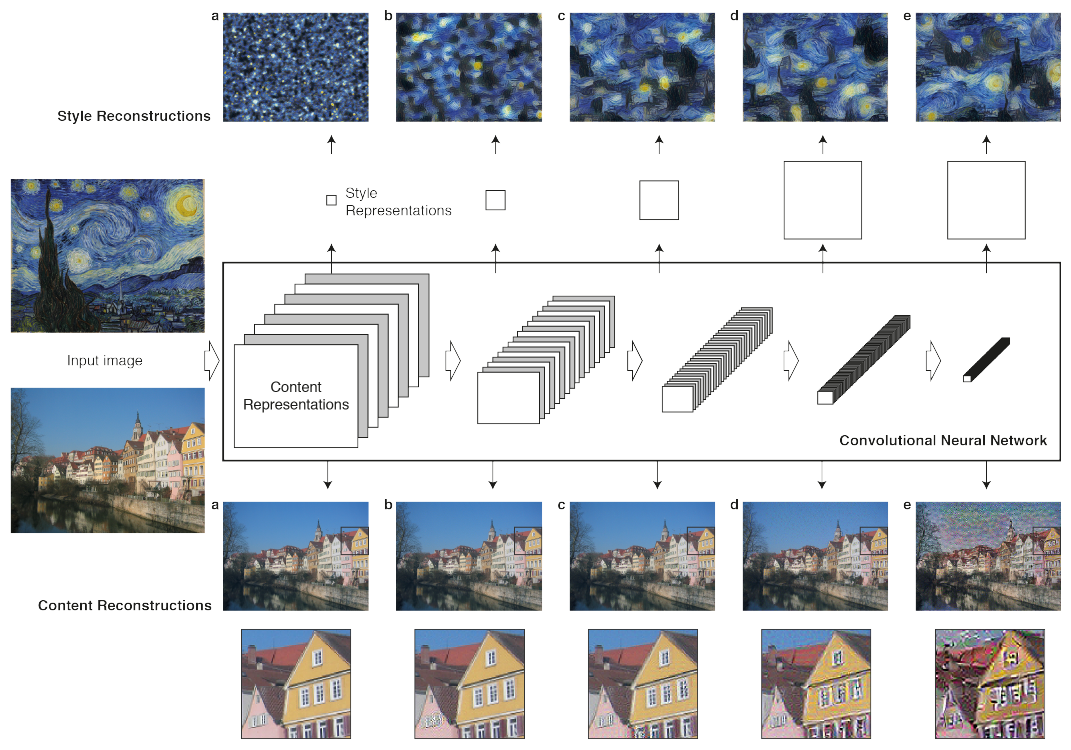
\includegraphics[width=\textwidth]{gfx/neural-style-cnn}
  \caption{
    Content and style reconstructions from an artwork and a photograph, respectively, using different feature maps from a CNN \cite{Gatys2015B}.
    As the input image gets processed by the CNN an increasing number of filter maps get produced in each layer.
    The totality of them for one layer are referred to in neural style as the content representation of the input image.
    At the bottom, content reconstructions of the photograph are generated at different stages of the VGG-Network from the following layers: ``conv1\_1'' (a), ``conv2\_1'' (b), ``conv3\_1'' (c), ``conv4\_1'' (d) and ``conv5\_1''.
    Style representations of an input image are built on top of content representations from a set of layers.
    At the top, style reconstructions of the artwork are generated using increasingly big subsets of layers: ``conv1\_1'' (a), ``conv1\_1'' and ``conv2\_1'' (b), ``conv1\_1'', ``conv2\_1'' and ``conv3\_1'' (c), ``conv1\_1'', ``conv2\_1'', ``conv3\_1'' and ``conv4\_1'' (d), ``conv1\_1'', ``conv2\_1'', ``conv3\_1'', ``conv4\_1'', and ``conv5\_1''.
    Including content representations from higher layers make the receptive field of style representations increase in size, and thus, the style reconstructions present larger local structures from the original artwork.
  }
  \label{sub:system:method:reconstructions}
\end{figure}


\subsection{Mixed Representation}
\label{sub:system:method:mixed-representation}

Having described how to separately reconstruct content and style from an original image it is straightforward to explain how the neural style algorithm is capable of simultaneously reconstructing both content and style from two different sources and producing the images in \autoref{sub:system:examples}.

Like in the previous cases, we want to find a new image $\vec{x}$ whose content representation and style representation matches at the same time the content representation of a photograph $\vec{p}$ in a given layer and the style representation of an artwork $\vec{a}$ in a set of layers.
Starting from a white noise image $\vec{x}$ the algorithm will simply need to minimize the following combined loss function:

\begin{equation}
  \mathcal{L}_{total}(\vec{p}, \vec{a}, \vec{x}) =
    \alpha \mathcal{L}_{content}(\vec{p}, \vec{x}) +
    \beta \mathcal{L}_{style}(\vec{a}, \vec{x})
\end{equation}

Where $\alpha/\beta$ is the ratio of emphasis of content over style, since content and style cannot be completely disentangled and a trade-off must be manually adjusted for each pair of source images.
The gradients $\Delta \vec{x}$, as before, are calculated with standard error propagation and are used to adjust the white noise image $\vec{x}$ until it reaches a compelling result.
The optimization process is one of huge dimensionality, taking into account the 144 million parameters in VGG-19 \cite{Simonyan2014}, and the unconstrained resolution of source images, and so \citeauthor{Gatys2015A} propose L-BFGS \cite{Zhu1994} as a suitable gradient optimization strategy.


% ------------------------------------------------------------------------------

\section{Results}
\label{sec:system:results}

\citeauthor{Gatys2015B} presented in \cite{Gatys2015B} a series of results to showcase how each different hyperparameter affect the outcome of the algorithm as they vary.
As hinted while explaining the reconstruction process, the hyperparameters taken into account are three: 1) the ratio of emphasis on content over style $\alpha / \beta$, 2) the relative weights given to the CNN layers for style representation $\vec{w}_L$, and 3) which CNN layer is used for content representation.

\autoref{fig:system:results} shows results of some variations arranged in a grid where columns show variation in emphasis on content over style and rows variation of relative weights for style representation, having content representation fixed to CNN layer ``conv4\_2'' of the VGG-Network.
Although the style reconstruction method allows for arbitrary relative weights, \citeauthor{Gatys2015B} fixed on a simpler approach only using increasingly higher CNN layers and giving them equal relative weights.
In such configuration, relative weights for active CNN layers is set to $w_l = 1/n$, being $n$ the number of active layers, and to $w_l = 0$ for the rest.
Active CNN layers for style reconstruction per row: A) only ``conv1\_1'' ($w_l = 1$), B) ``conv1\_1'' and ``conv2\_1'' ($w_l = 1/2$), C) ``conv1\_1'', ``conv2\_1'' and ``conv3\_1'' ($w_l = 1/3$), D) ``conv1\_1'', ``conv2\_1'', ``conv3\_1'' and ``conv4\_1'' ($w_l = 1/4$), and finally E) ``conv1\_1'', ``conv2\_1'', ``conv3\_1'', ``conv4\_1'', and ``conv5\_1'' ($w_l = 1/5$).

\begin{figure}[!tb]
  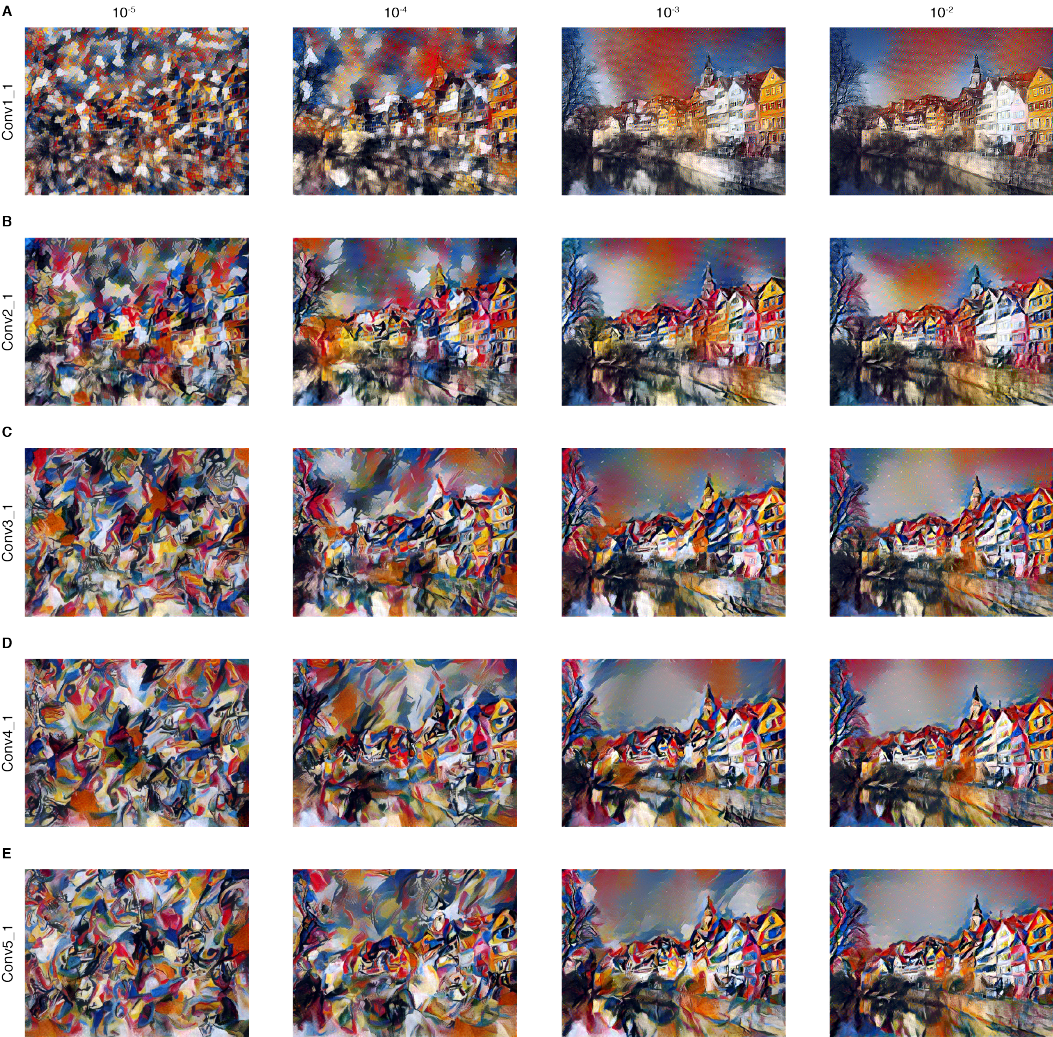
\includegraphics[width=\textwidth]{gfx/neural-style-results}
  \caption{
    Neural Style hyperparameter variation results of combining a photograph with the style of \emph{Composition VII} by Wassily Kandinsky.
    In the rows, from top to bottom, the increasing subset of CNN layers used for style representation, expressed with the higher layer used from VGG-Network (up to $conv\#\_1$).
    In the columns, from left to right, the increasing ratio $\alpha / \beta$ representing the emphasis on content over style.
    Including style features from higher layers of the network results in the style representation capturing bigger and more complex from the original artwork.
    Higher emphasis on content over style results in the synthesized image preserving more features of the original photograph.
  }
  \label{fig:system:results}
\end{figure}

Variations in emphasis on content over style show how increasing this ratio results on the features of the original photograph being preserved more faithfully.
If we look at \autoref{fig:system:results}~(A1), with a ratio of $10^{-5}$, very little is kept from the spatial information of the photograph and only some blue puffs representing the sky can be seen in the top region.
In \autoref{fig:system:results}~(A2), with a ratio of $10^{-4}$, the overall spatial arrangement of the photograph is already discernible, but, other than the closest building, the exact elements of the rest of the photograph are hard to tell.
Already in \autoref{fig:system:results}~(A3), with a ratio of $10^{-3}$, the buildings, river and tree are finally appreciable.
The exact spatial information remaining at the end is, however, dependent as well on the particular style representation chosen.

Now focusing on how the different style representations affect the outcome, we can see that including higher CNN layers makes the patterns increase in size and complexity.
The style representation captured ranges from showing little more than color puffs in \autoref{fig:system:results}~(A1), to similar shapes as seen in the original artwork in \autoref{fig:system:results}~(A5).
This makes sense if we think of CNNs trained in object recognition work.
Lower layers have small receptive fields and filters apply transformations that simply capture edges, corners or orientations.
On the other hand, higher layers have larger receptive fields due to subsampling and filters capture increasingly complex patterns such as shapes, text, or faces.

While Neural Style displays astounding capabilities for separation and mixing of style and content, compelling artistic results seem to be restricted to a particular region of hyperparameter values.
This region is not stationary as it varies from case to case depending on the photograph and artwork chosen and requiring careful fine-tuning of pixel fidelity (the chosen CNN layer for content representation), spatial information (the content-style ratio), and style representation complexity (the chosen CNN layers for style representation).


% ------------------------------------------------------------------------------

\section{Discussion}
\label{sec:system:discussion}

\citeauthor{Gatys2015B} are the first ones surprised with their results.
A neural system trained to perform a basic computational task of biological vision, such as object recognition, automatically learns image representations that allow successful separation of style and content.
They speculate that when learning object recognition, the network has to become invariant to all image variations that preserves object identity, and so the internal representations must help reach this goal.
Internal representations that capture not only the content of an image but also the possible variations in its appearance would be extremely practical for object recognition.

The style representation described for neural style, extracting correlations between neuron activations, although theorized by \citeauthor{Gatys2015A} with the sole intention of producing a statistical measure to characterize a texture, it is, in fact, a biologically possible.
Complex cells in the human primary human system, perform similar operations in order to perceive motion \cite{Adelson1985}, inviting to wonder if a process similar to neural style is what actually grants us the ability to abstract content from style and therefore our ability to create and enjoy art.

Yet, I argue we are still far from a method that encompasses the creativity process in the human mind.
\citeauthor{Gatys2015A} in \cite{Gatys2015A} regarded \citet{Portilla2000}'s approach in texture transfer as not grasping the whole scope of natural textures because the method required careful selection of statistical measurements on a per-texture basis in order.
This is not the case in neural style, as style and content are consistently separated.
However, images generated with neural style require fine-tuning hyperparameters to achieving compelling results on a per content-style pair basis.
How can we quantify aesthetic beauty? This is still an open problem in non-photorealistic rendering \cite{Ashikhmin2003} and although neural style appears to have brought us closer to answering it, there is more work to be done in that direction.

Neural style astonishing results attracted a lot of attention and a plenty of work is being done both directly adapting neural style for other purposes as well as applying the same concepts in different ways.
We will give a quick overview on this in the next chapter.
